\documentclass[11pt]{article}
\usepackage[margin=1in]{geometry}
\usepackage[T1]{fontenc}
\usepackage{lmodern,booktabs,tabularx,longtable,enumitem,xcolor,tikz}
\usepackage[hidelinks]{hyperref}
\usetikzlibrary{arrows.meta,positioning}
\definecolor{Forest}{HTML}{153C32}
\definecolor{Mint}{HTML}{C9F0DC}
\definecolor{Cream}{HTML}{F8F6EF}
\definecolor{Rust}{HTML}{B65738}
\hypersetup{colorlinks=true,linkcolor=Forest,urlcolor=Rust}
\setlist[itemize]{leftmargin=1.5em,itemsep=0.25em}
\setlist[enumerate]{leftmargin=1.7em,itemsep=0.35em}
\renewcommand{\arraystretch}{1.2}

\title{Digital Professor Integration Plan}
\author{Architecture, Course Knowledge, and Interaction Evidence}
\date{October 2026}

\begin{document}
\maketitle
\tableofcontents

\newpage
\section{Purpose and current priority}

The immediate goal is to align the team on the Digital Professor's overall architecture, module boundaries, responsibilities, inputs and outputs, persistent data, and handoffs. The system remains course-agnostic. Course-specific tutoring workflows and validation sets come later, after the component contracts are stable.

Two connected paths are central to the design:

\begin{itemize}
    \item \textbf{Document extraction, structured Course Context / Question Schema, and RAG} convert approved material into both verified system-wide structure and searchable course knowledge.
    \item \textbf{Interaction and Student Evidence} convert student input into a traceable record, retrieve relevant course context, coordinate tutoring decisions, deliver an action, and capture the student's response.
\end{itemize}

This phase should produce a component architecture, clear ownership boundaries, agreed handoff records, database schemas that support ingestion and retrieval, and a complete course-agnostic workflow. It should not commit the team to a particular framework, model provider, or deployment architecture.

\section{High-level architecture}

The architecture has two connected flows. The first prepares both searchable course material and structured course/question context. The second uses those outputs to interpret a student turn, update learner state, select a tutoring action, and deliver it.

\subsection{Course preparation and downstream consumers}

\begin{center}
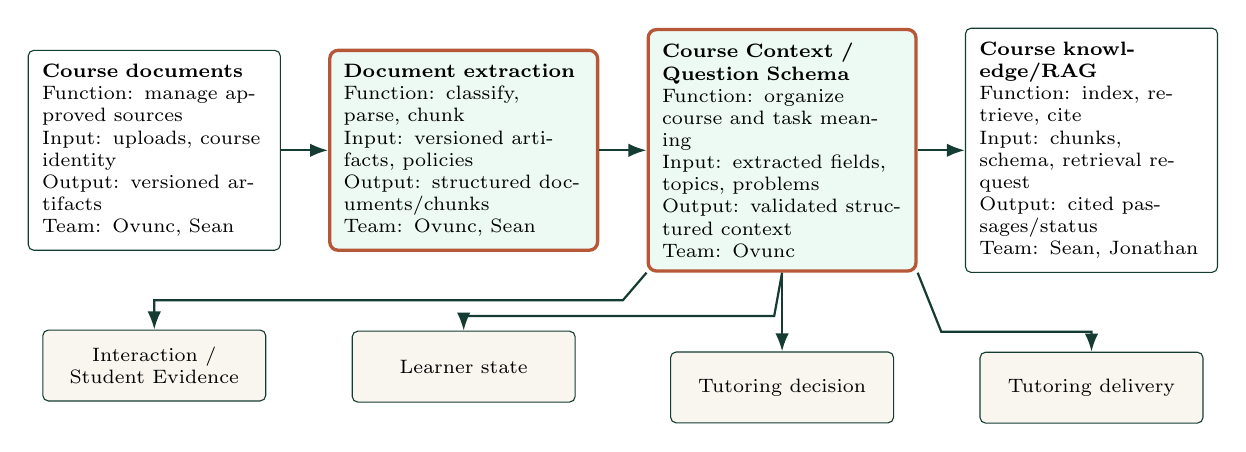
\begin{tikzpicture}[
  node distance=7mm and 6mm,
  box/.style={draw=Forest,rounded corners=2pt,fill=white,align=left,text width=2.85cm,minimum height=2.0cm,inner sep=5pt,font=\scriptsize},
  central/.style={draw=Rust,very thick,rounded corners=3pt,fill=Mint!35,align=left,text width=3.05cm,minimum height=2.0cm,inner sep=5pt,font=\scriptsize},
  consumer/.style={draw=Forest,rounded corners=2pt,fill=Cream,align=center,text width=2.55cm,minimum height=.9cm,inner sep=4pt,font=\scriptsize},
  arrow/.style={-{Latex[length=2.3mm]},thick,draw=Forest}]
\node[box] (docs) {\textbf{Course documents}\\Function: manage approved sources\\Input: uploads, course identity\\Output: versioned artifacts\\Team: Ovunc, Sean};
\node[central,right=of docs] (ingest) {\textbf{Document extraction}\\Function: classify, parse, chunk\\Input: versioned artifacts, policies\\Output: structured documents/chunks\\Team: Ovunc, Sean};
\node[central,right=of ingest] (context) {\textbf{Course Context / Question Schema}\\Function: organize course and task meaning\\Input: extracted fields, topics, problems\\Output: validated structured context\\Team: Ovunc};
\node[box,right=of context] (rag) {\textbf{Course knowledge/RAG}\\Function: index, retrieve, cite\\Input: chunks, schema, retrieval request\\Output: cited passages/status\\Team: Sean, Jonathan};
\node[consumer,below=10mm of docs] (interaction) {Interaction / Student Evidence};
\node[consumer,below=10mm of ingest] (state) {Learner state};
\node[consumer,below=10mm of context] (decision) {Tutoring decision};
\node[consumer,below=10mm of rag] (delivery) {Tutoring delivery};
\draw[arrow] (docs)--(ingest);
\draw[arrow] (ingest)--(context);
\draw[arrow] (context)--(rag);
\draw[arrow] (context.south west) -- ++(-.3,-.35) -| (interaction.north);
\draw[arrow] (context.south) -- ++(-.1,-.55) -| (state.north);
\draw[arrow] (context)--(decision);
\draw[arrow] (context.south east) -- ++(.3,-.75) -| (delivery.north);
\end{tikzpicture}
\end{center}

The structured context is not merely metadata for retrieval. It gives downstream modules a shared definition of the course, concept, question, expected response, prerequisites, source references, and assessment constraints. RAG supplies passages; the structured schema supplies stable meaning and relationships.

\subsection{Tutoring-turn flow}

\begin{center}
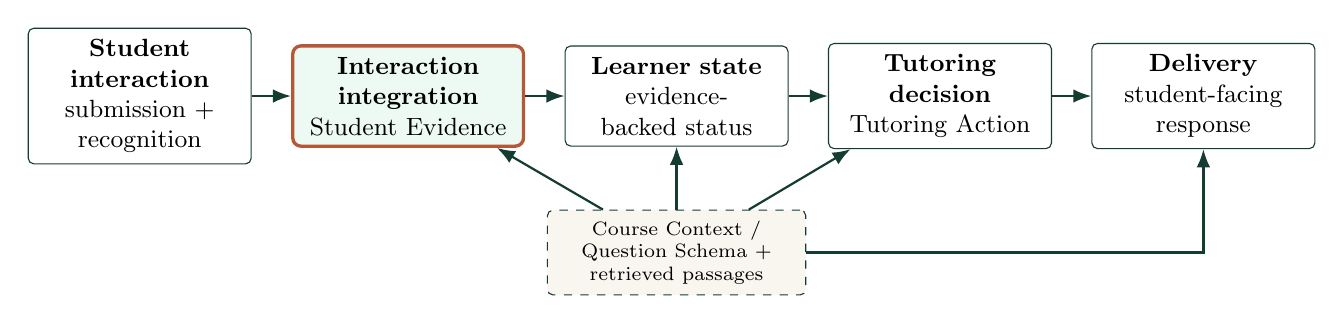
\begin{tikzpicture}[
  node distance=5mm,
  box/.style={draw=Forest,rounded corners=2pt,fill=white,align=center,text width=2.55cm,minimum height=1.25cm,inner sep=4pt,font=\small},
  central/.style={draw=Rust,very thick,rounded corners=3pt,fill=Mint!35,align=center,text width=2.65cm,minimum height=1.25cm,inner sep=4pt,font=\small},
  support/.style={draw=Forest,dashed,rounded corners=2pt,fill=Cream,align=center,text width=3.0cm,minimum height=.9cm,inner sep=4pt,font=\scriptsize},
  arrow/.style={-{Latex[length=2.3mm]},thick,draw=Forest}]
\node[box] (student) {\textbf{Student interaction}\\submission + recognition};
\node[central,right=of student] (evidence) {\textbf{Interaction integration}\\Student Evidence};
\node[box,right=of evidence] (state) {\textbf{Learner state}\\evidence-backed status};
\node[box,right=of state] (action) {\textbf{Tutoring decision}\\Tutoring Action};
\node[box,right=of action] (delivery) {\textbf{Delivery}\\student-facing response};
\node[support,below=8mm of state] (course) {Course Context / Question Schema + retrieved passages};
\draw[arrow] (student)--(evidence);
\draw[arrow] (evidence)--(state);
\draw[arrow] (state)--(action);
\draw[arrow] (action)--(delivery);
\draw[arrow] (course)--(evidence);
\draw[arrow] (course)--(state);
\draw[arrow] (course)--(action);
\draw[arrow] (course.east)-|(delivery.south);
\end{tikzpicture}
\end{center}

The state-to-action boundary is explicit: learner state reports what the evidence supports; tutoring decision applies the question schema, course constraints, and tutoring policy to choose what happens next. Delivery may use the same schema to render the problem, rubric-aware prompts, response controls, citations, or avatar behavior without changing the selected action.

\section{Module responsibilities}

Each module owns one part of the system. The boundary statements prevent two modules from silently making the same decision.

\noindent\begin{tabularx}{\textwidth}{@{}p{0.24\textwidth}X@{}}
\toprule
\textbf{Module} & \textbf{Responsibility and boundary} \\
\midrule
Course documents & Preserve approved syllabi, lecture notes, textbooks, problems, and other source files with stable identities and versions. This module owns original course artifacts, not extracted interpretations. \\
Document extraction & Register and classify sources; recover pages, structure, equations, tables, and course fields; create traceable chunks. It reports uncertainty rather than inventing missing content. \\
Course Context / Question Schema & Convert verified course structure and authored problems into stable, reusable records. It owns course, topic, prerequisite, question, expected-response, rubric, and source-reference meaning; it does not retrieve passages or judge a student's response. \\
Course knowledge/RAG & Index extracted chunks and retrieve ranked, approved course passages with page citations. It supplies grounding but does not diagnose the student or choose a tutoring action. \\
Student interaction & Capture and recognize text, handwriting, speech, images, equations, and files while preserving the original submission and asking for confirmation when meaning is ambiguous. \\
Interaction integration & Construct Student Evidence, request course context, route each turn, validate handoffs, and maintain the trace. It does not diagnose mastery or silently repair student work. \\
Learner state & Maintain an evidence-backed account of what the student has demonstrated, misconceptions, prerequisites, uncertainty, assistance, and unresolved needs. It does not select the next intervention. \\
Tutoring decision & Combine learner state, Student Evidence, Course Context, Question Schema, retrieved material, and tutoring policy to select the next question, hint, explanation, retry, comprehension check, or transfer action. \\
Tutoring delivery & Present the approved action through text, equations, avatar, speech, flashcards, or another channel without changing its pedagogical intent. \\
System configuration & Maintain course policies, tutoring rules, tool permissions, privacy settings, and delivery preferences that other modules require but do not produce. \\
Persistent state and trace & Store document versions, sessions, evidence, retrieval events, learner states, actions, and delivery history while preserving links and provenance. \\
\bottomrule
\end{tabularx}

\subsection{Structured Course Context and Question Schema}

\begin{tabularx}{\textwidth}{@{}p{0.23\textwidth}p{0.33\textwidth}X@{}}
\toprule
\textbf{Record} & \textbf{Core contents} & \textbf{Direct consumers} \\
\midrule
\texttt{CourseContext} & Course identity and version, term, overview, learning objectives, topic hierarchy, prerequisite graph, policies, assessment structure, and source references & RAG uses scope and filters; interaction identifies the course and concept; learner state uses objectives and prerequisites; tutoring decision applies policies; delivery displays course-aware labels and guidance. \\
\texttt{QuestionSchema} & Question ID and version, topic/objective links, prompt, expected response type, rubric or success criteria, difficulty, prerequisites, permitted assistance, source references, and delivery hints & Interaction binds evidence to the question; learner state compares evidence with expected work; tutoring decision chooses allowed support; delivery renders the prompt, response controls, feedback, or alternate channel. \\
\bottomrule
\end{tabularx}

These records contain verified structure rather than retrieved prose. A downstream module may consume them directly even when no RAG call is needed. Retrieved passages remain separately attributed supporting material.

\subsection{Main logical functions}

These names describe system responsibilities and do not require a particular language or service structure.

\noindent\begin{tabularx}{\textwidth}{@{}p{0.27\textwidth}X@{}}
\toprule
\textbf{Function} & \textbf{Purpose} \\
\midrule
\texttt{register\_document} & Store the original artifact, create its identity and version, and start a processing job. \\
\texttt{classify\_document} & Determine the document type and return confidence and alternatives. \\
\texttt{extract\_structure} & Recover pages, headings, paragraphs, equations, tables, and document-specific fields. \\
\texttt{build\_course\_}\allowbreak\texttt{context} & Create the verified course, topic, learning-objective, prerequisite, policy, and source-reference structure consumed across the system. \\
\texttt{validate\_question\_}\allowbreak\texttt{schema} & Check a question's identity, concept, prompt, expected response, rubric or criteria, difficulty, prerequisite links, permitted support, and source references. \\
\texttt{build\_chunks} & Create retrievable units with stable source locations and parent-child relationships. \\
\texttt{index\_course\_}\allowbreak\texttt{content} & Write chunks to vector and keyword indexes using the current embedding and index version. \\
\texttt{retrieve\_course\_}\allowbreak\texttt{context} & Apply course and document filters, retrieve candidates, rerank them, and return cited passages. \\
\texttt{receive\_submission} & Preserve student input and attach session, problem, modality, and turn context. \\
\texttt{confirm\_recognition} & Ask the student to resolve recognition alternatives that could change meaning. \\
\texttt{build\_student\_}\allowbreak\texttt{evidence} & Represent the student's confirmed work, explanation, uncertainty, revision, and prior assistance. \\
\texttt{update\_learner\_}\allowbreak\texttt{state} & Convert validated evidence into an evidence-backed state update without choosing an intervention. \\
\texttt{select\_tutoring\_}\allowbreak\texttt{action} & Apply the question schema, learner state, course context, retrieved passages, and tutoring rules to choose the next action. \\
\texttt{route\_tutoring\_turn} & Send validated evidence and course context to the correct state, decision, retrieval, and delivery components. \\
\texttt{deliver\_action} & Render an approved tutoring action and record what the student actually received. \\
\texttt{record\_turn\_trace} & Link submissions, evidence, retrieval, decisions, tool use, delivery, and responses. \\
\bottomrule
\end{tabularx}
\newpage
\section{Key inputs and outputs}

This table states the main contract for each module. Detailed field definitions appear later in the database and handoff sections.

\small
\noindent\begin{tabularx}{\textwidth}{@{}p{0.21\textwidth}p{0.34\textwidth}X@{}}
\toprule
\textbf{Module} & \textbf{Receives} & \textbf{Returns} \\
\midrule
Course documents & Uploaded source files, course association, and approval or replacement decision & Stable document/version IDs, original-artifact references, metadata, and availability status \\
Document extraction & Approved document version and extraction/chunking policy & Classification, structured pages, extracted fields, chunks, source locations, confidence, and warnings \\
Course Context / Question Schema & Verified extracted course fields, topic structure, authored problems, policies, and source references & Versioned \texttt{CourseContext} and \texttt{QuestionSchema} records with validation status \\
Course knowledge/RAG & Extracted chunks, index configuration, live query, course scope, and filters & Index status or ranked passages, parent context, page citations, scores, and insufficient-context status \\
Student interaction & Raw student input, channel capabilities, and current turn context & Submission, recognition candidates, uncertainty, confirmation status, and student response \\
Interaction integration & Submission, recognition, prior action, session context, and retrieved passages & Student Evidence, grounded turn context, routing request, and complete trace \\
Learner state & Student Evidence, prior state, Course Context, Question Schema, and retrieved context & Updated evidence-backed state, unresolved needs, and confidence/status \\
Tutoring decision & Learner state, Student Evidence, Course Context, Question Schema, retrieved passages, tutoring rules, and tools & Selected action, goal, constraints, sources, allowed support, and expected response \\
Tutoring delivery & Approved action, Course Context/Question Schema display fields, channel capabilities, and preferences & Presented problem or intervention, delivery status, and next-response link \\
System configuration & Course policies, team-approved tutoring rules, permissions, retention policy, and user preferences & Versioned constraints, available-tool list, and channel settings \\
Persistent state and trace & Validated records and events from every module & Prior session/learner state, linked history, active versions, and audit trace \\
\bottomrule
\end{tabularx}
\normalsize
\newpage
\section{Handoffs between components}

The system passes named records rather than loose text. The table below shows the direction and purpose of each major handoff.

\small
\noindent\begin{tabularx}{\textwidth}{@{}p{0.20\textwidth}p{0.24\textwidth}p{0.20\textwidth}X@{}}
\toprule
\textbf{Sender} & \textbf{Handoff} & \textbf{Receiver} & \textbf{Purpose} \\
\midrule
Course documents & Document/version record & Document extraction & Identify the approved, immutable source to process. \\
Document extraction & \texttt{StructuredDocument} & Course Context/Question Schema and Course knowledge/RAG & Supply classified pages, hierarchy, chunks, fields, equations, source locations, and warnings. \\
Course Context / Question Schema & \texttt{CourseContext} and \texttt{QuestionSchema} & RAG, interaction integration, learner state, tutoring decision, and delivery & Give every downstream module the same course, concept, problem, prerequisite, expected-response, rubric, policy, and source-reference meaning. \\
Interaction integration & \texttt{RetrievalRequest} & Course knowledge/RAG & Ask for course material scoped to the current turn. \\
Course knowledge/RAG & \texttt{RetrievedContext} & Interaction integration, learner state, and tutoring decision & Ground the turn with ranked passages and page citations, or report insufficient context. \\
Student interaction & \texttt{StudentSubmission} and \texttt{RecognitionResult} & Interaction integration & Supply original input, interpreted content, alternatives, uncertainty, and confirmation status. \\
Interaction integration & \texttt{StudentEvidence} and grounded turn & Learner state & Supply confirmed work, explanation, uncertainty, revisions, prior assistance, course/question identity, and retrieved sources. \\
Learner state & \texttt{LearnerState} & Tutoring decision & State what the evidence supports, assistance already used, unresolved needs, confidence, and prerequisite or misconception flags. \\
Tutoring decision & \texttt{TutoringAction} & Tutoring delivery & Specify the next approved action, goal, constraints, sources, permitted help, and expected response. \\
Tutoring delivery & \texttt{DeliveryResult} & Interaction integration & Record what the student received and connect the next response to that action. \\
System configuration & Policy and settings record & Interaction integration, learner state, tutoring decision, and delivery & Supply rules, permissions, tools, privacy constraints, and channel settings that are not produced by the preceding module. \\
Persistent state and trace & Prior-state and history records & Interaction integration, learner state, and tutoring decision & Restore prior state and accepted versions; receive validated records from all modules for storage. \\
\bottomrule
\end{tabularx}
\normalsize

Every handoff preserves its origin, status, and version. Student-authored content, recognition output, retrieved material, system interpretation, and tool output remain distinguishable.

\section{Supporting note: document extraction and RAG design}

This section records useful implementation-facing detail, but it is supporting material for the current milestone. The immediate design decision is the boundary between structured course/question context, searchable course knowledge, and their downstream consumers.

\subsection{Ingestion pipeline}

\begin{enumerate}
    \item \textbf{Register and preserve.} Store the original file, calculate a checksum, assign document and version identifiers, and associate it with a course only when that association is known.
    \item \textbf{Classify.} Identify the material as a syllabus, lecture notes, textbook, assignment, worked example, or other type. Preserve confidence and alternate classifications.
    \item \textbf{Extract.} Recover page text and layout. Apply OCR to image-only pages. Preserve equations, tables, headings, lists, page numbers, and reading order rather than flattening everything into one text block.
    \item \textbf{Normalize.} Remove repeated headers and footers, repair safe line-break artifacts, retain meaningful notation, and record transformations. Keep the raw extraction for comparison.
    \item \textbf{Structure.} Build a document hierarchy such as document, chapter, section, subsection, page, and content block. Extract syllabus-specific course fields without mixing those fields into lecture-note topic extraction.
    \item \textbf{Chunk.} Create retrieval units from the structure, attach complete metadata, and retain links to the larger parent section and original page.
    \item \textbf{Index.} Create embeddings, keyword-search entries, and filters for course, document type, document version, topic, section, and page.
    \item \textbf{Validate and publish.} Check extraction coverage, empty or duplicate chunks, missing page links, broken equations, and index counts. Only approved document versions become available to retrieval.
\end{enumerate}

\subsection{Chunking strategy}

Chunking should follow document meaning before token count. The initial policy should support separate rules by material type:

\begin{itemize}
    \item \textbf{Syllabi:} use semantic sections such as overview, learning outcomes, schedule, assessment, and policies. Store structured fields separately and link each field to its source chunk and page.
    \item \textbf{Lecture notes:} chunk by heading and coherent explanation or worked step. Keep a theorem with its conditions, an equation with its definitions, and a worked example with the steps needed to interpret it.
    \item \textbf{Textbooks:} use a parent-child design. Small child chunks support precise retrieval; larger section or subsection parents restore context after retrieval.
    \item \textbf{Equations and tables:} store a normalized representation plus nearby explanatory text and the original page region. Do not separate symbols from their definitions.
    \item \textbf{Size and overlap:} begin with moderate child chunks, roughly 300--700 tokens, and small overlap only where a boundary divides a continuing explanation. Measure the actual distribution instead of forcing every chunk to the same size.
    \item \textbf{Traceability:} every chunk retains course, document, version, type, hierarchy path, page range, character or block offsets, and parent identifiers.
\end{itemize}

\subsection{Setting up retrieval for success}

\begin{itemize}
    \item Index only approved document versions and prevent cross-course retrieval by default.
    \item Combine semantic vector search with keyword or lexical search so exact course terms, theorem names, symbols, and policy wording remain findable.
    \item Apply metadata filters before or during retrieval, including course, term, document type, topic, and active version.
    \item Retrieve a broad candidate set, rerank it for the current question, and return a small set of passages with page-level citations.
    \item Expand a selected child chunk with its parent or neighboring chunks when the local passage lacks definitions or necessary steps.
    \item Preserve the retrieval query, filters, candidate scores, reranking result, index version, and returned chunk IDs in the turn trace.
    \item Return an explicit insufficient-context result when the knowledge base does not support the request. The tutoring model must not invent course-specific claims.
    \item Re-index deterministically when parsing, chunking, embedding, or source versions change; keep old traces tied to the index version that produced them.
\end{itemize}

\section{Supporting note: persistent data and database schemas}

This section preserves a possible persistence model for later refinement. The current milestone requires agreement on record meaning and ownership; exact tables, field types, and storage technologies can remain provisional.

A relational database should hold identity, state, provenance, and relationships. A vector index should hold embeddings keyed to relational chunk IDs. Original artifacts belong in file or object storage. These may be deployed together for a prototype, but their logical responsibilities should remain separate.

\small
\begin{longtable}{@{}p{0.19\textwidth}p{0.34\textwidth}p{0.37\textwidth}@{}}
\toprule
\textbf{Table or store} & \textbf{Core fields} & \textbf{Purpose and relationships} \\
\midrule
\endhead
\texttt{courses} & \texttt{course\_id}, name, number, term, overview, status & Root scope for documents, sessions, retrieval, and course configuration. \\
\texttt{course\_contexts} & context ID, course/version IDs, objectives, topic and prerequisite graph, policies, assessment structure, source links, status & Stable structured course meaning shared directly with interaction, learner state, tutoring decisions, delivery, and retrieval. \\
\texttt{question\_schemas} & question ID, context/topic IDs, prompt, expected response type, rubric or criteria, difficulty, prerequisites, permitted support, source links, version & Defines a question independently of any one delivery channel or student attempt. \\
\texttt{documents} & \texttt{document\_id}, course ID, type, title, source URI, checksum, active version & Stable identity for each syllabus, note set, textbook, assignment, or example. \\
\texttt{document\_versions} & \texttt{version\_id}, document ID, file URI, parser version, status, created time & Keeps ingestion reproducible and prevents a replaced file from changing old traces. \\
\texttt{pages} & \texttt{page\_id}, version ID, page number, raw text, normalized text, image URI & Page-level source and display unit. \\
\texttt{sections} & \texttt{section\_id}, version ID, parent section ID, heading, level, page range & Document hierarchy used by chunking and context expansion. \\
\texttt{chunks} & \texttt{chunk\_id}, version, section and page IDs, text, token count, offsets, parent chunk ID, metadata & Canonical retrievable unit and citation target. \\
Vector index & \texttt{chunk\_id}, embedding, embedding model/version, searchable metadata & Semantic retrieval; the chunk ID resolves to authoritative content in the relational store. \\
Keyword index & \texttt{chunk\_id}, indexed text and fields & Exact-term and lexical retrieval used alongside vector search. \\
\texttt{ingestion\_jobs} & job ID, version ID, stage, status, warnings, metrics, start/end time & Tracks extraction, chunking, indexing, failures, and approval. \\
\texttt{retrieval\_events} & retrieval ID, turn ID, query, filters, index version, candidate and returned chunk IDs, scores & Makes every grounded response reproducible and inspectable. \\
\texttt{sessions} and \texttt{turns} & session/turn IDs, course ID, student reference, problem context, times, status & Orders the interaction and connects it to the correct course scope. \\
\texttt{submissions} & submission ID, turn ID, modality, raw artifact URI, entered text, timestamp & Immutable record of what the student provided. \\
\texttt{recognition\_}\allowbreak\texttt{results} & result ID, submission ID, candidate content, alternatives, uncertainty, provider/settings & Separates machine recognition from confirmed student content. \\
\texttt{student\_evidence} & evidence ID, turn ID, confirmed content, steps, explanation, uncertainty, prior action, revision link, status & Canonical evidence passed to learner state and tutoring decision. \\
\texttt{learner\_states} & state ID, session ID, concept statuses, misconceptions, prerequisites, evidence links, version & Evidence-backed state at a point in the interaction. \\
\texttt{tutoring\_actions} & action ID, turn ID, type, goal, content constraints, source and tool links, expected response & Decision output independent of presentation channel. \\
\texttt{delivery\_events} & delivery ID, action ID, channel, rendered content, status, timing & Records what the student actually saw or heard. \\
\bottomrule
\end{longtable}
\normalsize

All stored records need stable IDs, timestamps, producer or source, status, and schema or model version where applicable. Foreign keys should enforce course, document, session, turn, and revision relationships. Deleting or replacing a derived record must not erase the original course file or student submission.

\section{Complete workflow: what enters, leaves, and is tracked}

\subsection{Course setup workflow}

\noindent\begin{tabularx}{\textwidth}{@{}p{0.23\textwidth}p{0.34\textwidth}X@{}}
\toprule
\textbf{Stage} & \textbf{Returns} & \textbf{Tracks} \\
\midrule
Register course document & Document and version IDs; stored-artifact reference; processing status & Checksum, storage location, uploader, course association, time, and approval state \\
Classify and extract & Document type; pages; hierarchy; equations; tables; extracted course fields & Parser/OCR versions, confidence, alternatives, warnings, and transformations \\
Build structured course/question context & Validated \texttt{CourseContext} and \texttt{QuestionSchema} records & Topic and prerequisite links, expected response, rubric/criteria, difficulty, policies, permitted support, sources, author, version, and validation status \\
Build chunks & Linked chunks ready for indexing & Section hierarchy, page range, offsets, token count, overlap, parent links, and chunking-policy version \\
Build indexes & Vector and keyword entries; index version; indexing status & Embedding model/version, rejected chunks, searchable metadata, and completion counts \\
Publish course knowledge & Retrieval-ready and coverage status & Active document/index versions and missing, failed, or superseded material \\
\bottomrule
\end{tabularx}

\subsection{Tutoring-turn workflow}

\noindent\begin{tabularx}{\textwidth}{@{}p{0.23\textwidth}p{0.34\textwidth}X@{}}
\toprule
\textbf{Stage} & \textbf{Returns} & \textbf{Tracks} \\
\midrule
Capture student input & Accepted submission and immutable artifact reference & Session, problem, modality, turn, timestamp, and current delivery/action link \\
Recognize and confirm & Candidate content, alternatives, uncertainty, and confirmed interpretation & Provider, settings, latency, candidate history, and student correction effort \\
Build Student Evidence & Validated work, steps, explanation, uncertainty, and revision & Provenance, prior assistance, attempt/revision links, and validation status \\
Apply course/question context & Turn context with stable course, concept, question, prerequisite, expected-response, rubric, and source identities & Context/schema versions and which fields were supplied to each downstream module \\
Retrieve course context & Ranked course passages or insufficient-context status & Query, filters, index version, candidates, scores, selected chunks, and citations \\
Update learner state & Evidence-backed current state & Evidence supporting each conclusion, misconceptions, prerequisites, help, and unresolved issues \\
Select tutoring action & One approved question, hint, explanation, retry, check, or transfer action & Pedagogical goal, constraints, sources, tools, rules, and expected response \\
Deliver action & Presented content and delivery status & Exact content, channel, timing, interruptions, preferences, and action link \\
Capture next response & New submission and turn linked to the action & Full path from course sources and evidence through decision, delivery, and revision \\
\bottomrule
\end{tabularx}

\subsection{Learner state to tutoring action}

The learner-state record describes the student without prescribing the intervention. The tutoring-decision component combines that state with the current Question Schema, Course Context, retrieved passages, and tutoring policy. This separation allows decision rules to change without rewriting the evidence history.

\noindent\begin{tabularx}{\textwidth}{@{}p{0.27\textwidth}p{0.32\textwidth}X@{}}
\toprule
\textbf{Learner-state signal} & \textbf{Question-schema constraint} & \textbf{Possible effect on Tutoring Action} \\
\midrule
Evidence is sufficient and correct & Required reasoning and response type are satisfied & Confirm briefly, then choose a comprehension or transfer check. \\
Partially correct step or local misconception & Rubric identifies the missing criterion or step & Ask a targeted question or give a bounded hint tied to that criterion. \\
Wrong approach & Expected method or concept relationship conflicts with the attempt & Surface the mismatch and request a revised approach without silently solving the task. \\
Missing prerequisite & Question lists a prerequisite not yet demonstrated & Run a prerequisite check or short review before returning to the current question. \\
Insufficient evidence & Expected response requires reasoning, work, or an explanation that is absent & Request the missing work rather than infer mastery from an answer alone. \\
High uncertainty or repeated difficulty & Assistance limit, retry count, or escalation rule is reached & Change strategy, reduce step size, explain more directly, or request human review. \\
\bottomrule
\end{tabularx}

\section{Things to agree on}

\begin{itemize}
    \item The final module list, the owner of each module, and the owner of every handoff.
    \item Which document types enter the first course knowledge base and who approves a document version.
    \item The extraction output required for syllabi, lecture notes, textbooks, equations, and tables.
    \item The minimum contents, ownership, authoring process, and validation rules for \texttt{CourseContext} and \texttt{QuestionSchema}.
    \item Which structured course/question fields RAG, interaction integration, learner state, tutoring decision, and delivery each consume directly.
    \item Initial chunking policies by document type, including hierarchy, size, overlap, and parent expansion.
    \item Vector, keyword, and reranking responsibilities and the minimum metadata required for filtering and citation.
    \item The minimum fields in each database table and handoff record, plus versioning and retention rules.
    \item Where Student Evidence ends, what learner state may infer, and what information tutoring decision must use before selecting an action.
    \item When recognition ambiguity must return to the student for confirmation.
    \item What each component returns when extraction, retrieval, recognition, a tool, or delivery fails.
\end{itemize}

\section{Things to do and proposed collaboration}

\begin{enumerate}
    \item \textbf{Ovunc and Sean:} define the syllabus and lecture ingestion path from uploaded file through structured documents, structured course/question context, chunks, indexes, and retrieval-ready status.
    \item \textbf{Ovunc:} define \texttt{CourseContext} and \texttt{QuestionSchema}, including topics, prerequisites, learning objectives, prompt, expected response, rubric/criteria, difficulty, policies, permitted support, and source references.
    \item \textbf{Sean:} specify chunking, embeddings, hybrid retrieval, reranking, filters, citations, index versioning, and the knowledge-base database needs.
    \item \textbf{Sean and Jonathan:} agree on what retrieval receives from structured context and a student turn, and what grounded context returns to Student Evidence, learner state, and tutoring decision.
    \item \textbf{Ovunc and Jonathan:} define how Question Schema and Student Evidence combine to update learner state, then specify the learner-state-to-tutoring-action contract.
    \item \textbf{Jonathan:} define Student Evidence, interaction routing, trace records, learner-state updates, and the handoffs connecting recognition, structured context, retrieval, decisions, and delivery.
    \item \textbf{Ovunc and Yining Li:} identify the Course Context and Question Schema fields delivery needs to render questions, response controls, feedback, flashcards, speech, and avatar behavior consistently.
    \item \textbf{Yining Li:} define how a selected tutoring action is expressed through each channel and how the student's response returns to interaction integration.
    \item \textbf{Whole team:} review the database schema and one complete course-setup and tutoring-turn walkthrough; resolve missing fields, duplicated responsibility, and unclear failure handling.
    \item Freeze architecture and interface version 0.1 before choosing detailed APIs or implementing deeper module internals.
\end{enumerate}

\section{Future work}

After architecture and contracts stabilize, the team can:

\begin{itemize}
    \item create a small Calculus tutoring workflow and example set to validate the integrated design;
    \item define formal evaluation criteria for extraction, retrieval, Student Evidence, grounding, tutoring decisions, and delivery;
    \item compare chunking, embedding, retrieval, reranking, recognition, and model alternatives;
    \item measure retrieval quality, response reliability, latency, cost, and correction effort;
    \item expand course-specific workflows while keeping the shared architecture course-agnostic; and
    \item implement broader avatar and real-time interaction support.
\end{itemize}

The present milestone is complete when the team can trace an uploaded course document into structured Course Context, Question Schema, and the searchable knowledge base, then trace a student turn through evidence, learner state, tutoring action, and delivery, with a clear owner, input, output, stored record, and failure result at every step.

\end{document}
